\section{B1. Approches techniques}

	L'intérêt du web offline est de permettre à un utilisateur d’utiliser ses applications habituellement connectées à internet (boite mail, streaming musical …) ou de consulter ses pages web préférées (casisbelli …), le tout, en étant hors-ligne. Cette technologie s’est principalement développée grâce à l’augmentation du nombre de smartphones et de tablettes. \\

	Afin de pouvoir utiliser un site web ou une application hors ligne, nous devons connaître l’état de connexion de l’utilisateur, c’est-à-dire, savoir s’il est connecté à internet ou non \textit{(pattern Message Endpoint)}. Cette étape est généralement réalisée à l’aide de fonctions de type javascripts en utilisant notamment : navigator.onLine. Une fois que nous avons pris connaissance de l’état de connexion de l’utilisateur, nous devons spécifier quelles sont et où sont situés les informations nécessaires afin d’afficher correctement le site internet ou le contenu de l’application. Cette étape passe généralement par la création d’un fichier appelé Cache Manifest et enregistré généralement sous le nom offline.manifest. Voici un exemple de fichier :\\

	CACHE MANIFEST\\
	angular.min.js\\
	bootstrap.min.js\\
	styles-perso.css\\
	jquery-1.4.min.js\\
	offline.js\\
	index.html\\
	exercices.html\\
	contact.html\\

	Il faut ensuite lier ce Cache Manifest à nos pages html de la manière suivante : \textit{$<html manifest="offline.manifest">$}\\

	Il est important de noter que les exemples donnés ci-dessus et par la suite de cette partie reposent sur l’utilisation de la technologie Application Cache. Il existe une autre technologie nommée Service Worker que nous développerons dans la partie suivante.\\

	Ensuite, il est important de stocker les données localement afin d’avoir accès aux données et de pouvoir utiliser correctement le site web ou l’application \textit{(pattern Message Store)}. \\

	Pendant l’utilisation, il est nécessaire de veiller à enregistrer les données régulièrement dans la base de données locale au risque de perdre des données dans le cas contraire. La solution la plus simple à mettre en place est la sauvegarde du DOM des pages web à l’aides des objets suivants :

	\begin{itemize}
		\item window.sessionStorage pour sauvegarder pendant la période de Session
		\item window.localStorage pour sauvegarder pour une période plus importante
	\end{itemize}
	~\\

	Dans tous les cas, ces objets offrent le même type de fonction permettant d'accéder aux données, de sauvegarder ces dernières ou de les supprimer facilement.\\

	Une fois que la connexion à internet est rétablie, les données stockées en locale doivent être synchronisées avec le serveur distant \textit{(pattern Messaging)} \textit{(pattern Message Endpoint)} \textit{(pattern Message Filter)}. Il faut donc prévoir de créer une queue des données pour être cohérent avec l’évolution des données en mode hors ligne \textit{(pattern Resequencer)}. La transaction des données doit être vérifiée et réussie pour pouvoir passer à la transaction suivante \textit{(pattern Guaranteed Delivery)}. Si la connexion à internet coupe pendant une transaction, c’est comme ci elle n’avait pas été réalisée et doit donc être refaite lors d’une nouvelle connexion à internet. De plus, si des modifications ont été réalisées sur le serveur distant entre deux connexions, ces dernières vont être téléchargées vers le dossier de stockage local \textit{(pattern Shared Database)}.

\section{B2. Solutions technologiques}

\section{B3. Description technique}

\section{B4. Benchmark}

\section{B5. Work Breakdown Structure}

 \begin{figure}[H]
 \centering
  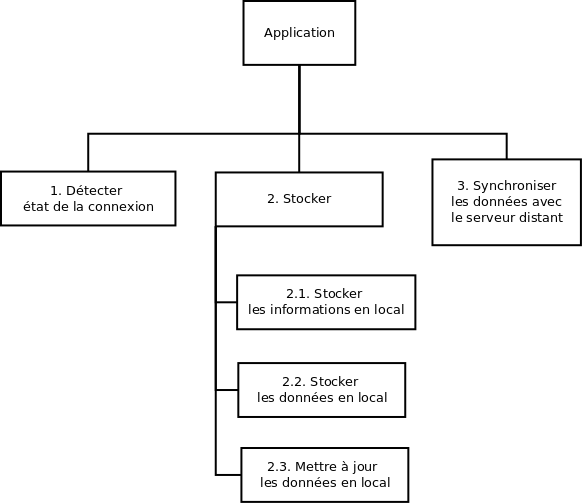
\includegraphics[width=18cm]{./images/wbs.png}
\caption{Work Breakdown Structure}
  \end{figure}
